\section{Análisis de Estacionalidad}

Estacionariedad significa que el conjunto de datos debería tener una media, varianza y covarianza constante.

Para descubrir si este conjunto es estacionario, se inicia por crear una representación gráfica de los datos de $train$ como del $test$, con el fin de observar su comportamiento. Esto se encuentra en la siguiente figura.


\begin{figure}[!h]
	\centering
	\includegraphics[width=0.7\linewidth]{gráfica_train_test_og}
	\caption{Gráfico de Train y Test}
	\label{fig:graficatraintestog}
\end{figure}

A simple vista se pueden sacar las siguientes conclusiones:
\begin{enumerate}
	\item Existe una tendencia ascendente a lo largo del tiempo, lo que indica un crecimiento en la serie
	\item La varianza es relativamente estable, aunque hay algunas fluctuaciones. La media no es constante debido a la tendencia creciente.
	\item La serie parece ser heterocdástica, ya que la variabilidad cambia a lo largo del tiempo aunque de manera gradual
	\item La serie no es estacionaria, dado que tanto la media como la variabilidad presentan cambios a lo largo del tiempo
	\item La serie presenta estacionalidad, ya que exhice un patrón recurrente en ciertos periodos, lo que sugiere la existencia de ciclos repetitivos.
\end{enumerate}


\subsection{Descomposición de la Serie Temporal}

Un conjunto de datos que fluctue alrededor de la tendencia y además, presenta valores homogéneos, suele tener como preferencia un esquema aditivio.
El siguiente código presenta el calculo de descomposición estacional.
\begin{lstlisting}
	result = seasonal_decompose(train["Sales"], model = "additive")
\end{lstlisting}



\begin{figure}[h]
	\centering
	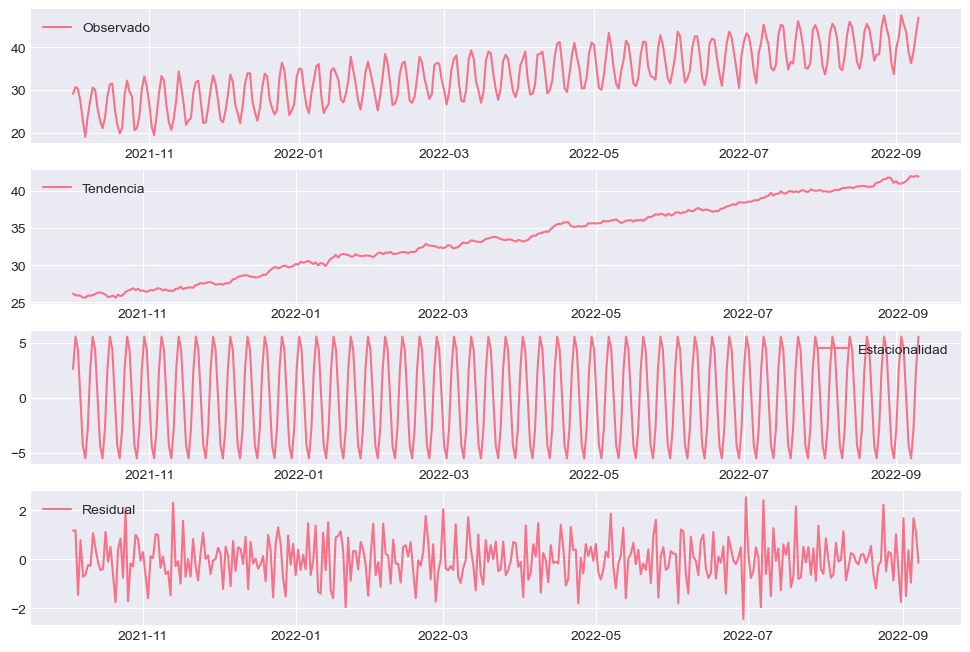
\includegraphics[width=0.7\linewidth]{seasonal_decompose_plot}
	\caption{Descomposición Estacional}
	\label{fig:seasonaldecomposeplot}
\end{figure}

La figura anterior muestra la descomposición de la serie temporal en sus componentes principales.
\begin{enumerate}
	\item	Serie Observada
	\begin{itemize}
		\item Presenta un patrón cíclico con variaciones periódicas
		\item Hay una tendencia alcista
	\end{itemize}
	\item Tendencia
	\begin{itemize}
		\item Muestra un incremento gradual y sostenido en el tiempo
		\item Hay momentos de suavización en el crecimiento, lo que puede indicar cambios en el comportamiento de la variable
	\end{itemize}
	\item Estacionalidad
	\begin{itemize}
		\item Hay un patrón repetitivo claro, lo que confirma que la serie es estacional.
		\item  La amplitud parece relativamente constante (-5, +5), lo que indica que la variabilidad estacional no cambia drásticamente
	\end{itemize}
	\item Residuo
	\begin{itemize}
		\item Representa las fluctuaciones no explicadas por la tendencia y la estacionalidad
		\item Hay variabilidad pero no hay un patrón claro, lo que sugiere que la descomposición ha capturado bien los componentes principales
		\item Algunos picos son más elevados, esto puede indicar valores atípicos
	\end{itemize}
\end{enumerate}

